\documentclass{article}

% Language setting
% Replace `english' with e.g. `spanish' to change the document language
\usepackage[russian]{babel}

% Set page size and margins
% Replace `letterpaper' with `a4paper' for UK/EU standard size
\usepackage[a4paper,top=2cm,bottom=2cm,left=3cm,right=3cm,marginparwidth=1.75cm]{geometry}

% Useful packages
\usepackage{amsmath, amssymb, amsthm}
\usepackage{indentfirst}
\usepackage{graphicx, float}
\usepackage[colorlinks=true, allcolors=blue]{hyperref}
\setlength{\parskip}{5pt}
\setlength{\parindent}{20pt}
\title{Эмпирические байесовские нейронные сети}
\author{Басов Дмитрий Константинович}
\date{}
\begin{document}
\maketitle

\begin{abstract}
Данная статья посвящена применению техники эмпирического Байеса к байесовским нейронным сетям. Концептуально идея следующая:
\begin{enumerate}
 \item Мы используем диагональное нормальное распределение для аппроксимации апостериорного распределения параметров модели~--- $q(W)$.
 \item Априорное распределение параметров модели так же задаётся диагональным распределением с нулевым матожиданием~--- $p(W)$.
 \item Используя вариационный вывод, мы приходим к ситуации, когда ELBO зависит от $KL(q(W) || p(W))$. Так как оба распределения являются нормальными, то KL дивергенция считается аналитически.
 \item Мотивация следующего этапа была взята из RVM~--- взять дисперсию априорного распределения параметров модели $p(W)$ из данных. Там несложно берётся производная и всё получается красиво, кроме возможного деления 0/0. Но сделав замену переменных, от этой беды можно уйти.
\end{enumerate}
Пункты 1--3 в принципе были описаны в статье \href{https://arxiv.org/pdf/1505.05424}{Weight Uncertainty in Neural Networks}. А вот четвёртый пункт я ни в книгах, ни в статьях не находил.

\end{abstract}


\section{Обозначения и сокращения}
$N(\mu, \sigma^2)$ — нормальное распределение

$\mathbf{x} \cdot \mathbf{y}$ — поэлементное произведение (произведение Адамара) векторов

$\mathcal{L}$ — Evidence Lower Bound (ELBO)

$KL(q || p) = \int_{}{} q(\mathbf{Z}) \cdot \ln{\dfrac{q(\mathbf{Z})}{p(\mathbf{Z})}} d\mathbf{Z}$ — расстояние Кульбака — Лейблера

$\mathbf{x}$ — вектор признаков

$\mathbf{y}$ — вектор целевой переменной

$D$ — датасет — пары значений \{$\mathbf{x_i}$, $\mathbf{y_i}$\}, где $i = 1, \dots, L$

$\mathbf{W}$ — параметры модели — случайная величина размерности M

$p(D | \mathbf{W}) = \prod_{i=1}^{L} p(\mathbf{y_i} | \mathbf{x_i}, \mathbf{W})$ — правдоподобие (likelihood)

$p(\mathbf{W})$ — априорное распределение параметров модели (prior)

$p(\mathbf{W}| D)$ — апостериорное распределение параметров модели (posterior)

$p(D)$ — маргинальная вероятность датасета (evidence)

$q(\mathbf{W})$ — аппроксимация апостериорного распределения параметров модели

$p(\mathbf{W}, D) =
p(D | \mathbf{W}) \cdot p(\mathbf{W}) =
p(\mathbf{W}| D)\cdot p(D)$
— совместная вероятность параметров и данных

\section{Постановка задачи}
Постановка задачи следующая: у нас есть датасет $D$ и наша цель — смоделировать распределение $p(\mathbf{y} | \mathbf{x}, D)$. То есть мы хотим получить распределение вероятностей целевой переменной $\mathbf{y}$ для неразмеченных $\mathbf{x}$, используя датасет D. Сделаем следующие преобразования:

$p(\mathbf{y} | \mathbf{x}, D) =
\int_{}{} p(\mathbf{y}, \mathbf{W} | \mathbf{x}, D) d\mathbf{W} =
\int_{}{} p(\mathbf{y} | \mathbf{W}, \mathbf{x}, D) \cdot p(\mathbf{W} | \mathbf{x}, D) d\mathbf{W} =
\int_{}{} p(\mathbf{y} | \mathbf{W}, \mathbf{x}) \cdot p(\mathbf{W} | D) d\mathbf{W}$

Получим выражение для $p(\mathbf{W}| D)$, используя формулу Байеса:

$p(\mathbf{W}| D) =
\dfrac{p(\mathbf{W}, D)}{p(D)} =
\dfrac{p(\mathbf{W}, D)}{\int_{}{} p(\mathbf{W}, D) d\mathbf{W}} =
\dfrac{p(D | \mathbf{W}) \cdot p(\mathbf{W})}{\int_{}{} p(D | \mathbf{W}) \cdot p(\mathbf{W}) d\mathbf{W}} $

Для аппроксимации распределения ответов модели можно воспользоваться методом Монте — Карло: взять сэмпл весов $\hat{\mathbf{W}}$ из $p(\mathbf{W}| D)$, и используя $\hat{\mathbf{W}}$ и $\mathbf{x}$, получить $\hat{\mathbf{y}}$. Однако для этого необходимо уметь сэмплировать из распределения $p(\mathbf{W}| D)$.

Получить аналитическое решение можно только в очень ограниченном числе случаев. Существует возможность сэмплировать из $p(\mathbf{W}| D)$, используя методы Монте — Карло для марковских цепей (MCMC). Однако для больших датасетов и большого числа параметров это практически невозможно. Альтернативный подход к решению таких задач — аппроксимация распределения $p(\mathbf{W}| D)$ распределением $q(\mathbf{W})$, из которого сэмплировать намного проще.


\section{Вариационный вывод для нейронной сети}
Запишем выражение ELBO для распределения $q(\mathbf{W})$ и преобразуем его, используя тождество $p(\mathbf{W}, D) = p(\mathbf{W}| D)\cdot p(D)$:

$
\mathcal{L}(q(\mathbf{W})) =
\int_{}{} q(\mathbf{W}) \cdot \ln{\dfrac{p(\mathbf{D}, \mathbf{W})}{q(\mathbf{W})}} d\mathbf{W} =
\int_{}{} q(\mathbf{W}) \cdot \ln{\dfrac{p(\mathbf{W}| D) \cdot p(D)}{q(\mathbf{W})}} d\mathbf{W} =
\ln{p(D)} \cdot \int_{}{} q(\mathbf{W}) d\mathbf{W} - \int_{}{} q(\mathbf{W})\cdot \ln{\dfrac{q(\mathbf{W})}{p(\mathbf{W}| D)}} d\mathbf{W} =
\ln{p(D)} - KL(q(\mathbf{W}) || p(\mathbf{W}| D))
$

Из равенства $\mathcal{L}(q(\mathbf{W})) = ln(p(D)) - KL(q(\mathbf{W}) || p(\mathbf{W}| D))$ видно, что максимизируя $\mathcal{L}(q(\mathbf{W}))$, мы не только максимизируем $\ln {p(D)}$, но и минимизируем $KL(q(\mathbf{W}) || p(\mathbf{W}| D))$. То есть распределение $q(\mathbf{W})$ будет приближаться к распределению $p(\mathbf{W}| D)$.

Будем максимизировать $\mathcal{L}(q(\mathbf{W}))$. Преобразуем выражение для $\mathcal{L}(q(\mathbf{W}))$, используя тождество
$p(\mathbf{W}, D) = p(D | \mathbf{W}) \cdot p(\mathbf{W})$:

$
\mathcal{L}(q(\mathbf{W})) =
\int_{}{} q(\mathbf{W}) \cdot \ln{\dfrac{p(\mathbf{D}, \mathbf{W})}{q(\mathbf{W})}} d\mathbf{W} =
\int_{}{} q(\mathbf{W}) \cdot \ln{\dfrac{p(D | \mathbf{W}) \cdot p(\mathbf{W})}{q(\mathbf{W})}} d\mathbf{W} =
\int_{}{} q(\mathbf{W}) \cdot \ln{p(D | \mathbf{W})} d\mathbf{W} - \int_{}{} q(\mathbf{W}) \cdot \ln{\dfrac{q(\mathbf{W})}{p(\mathbf{W})}} =
\int_{}{} q(\mathbf{W}) \cdot \ln{p(D | \mathbf{W})} d\mathbf{W} - KL(q(\mathbf{W}) || p(\mathbf{W}))
$

Для дальнейшнего вывода положим, что распределения $p(\mathbf{W})$ и $q(\mathbf{W})$ являются нормальными с диагональными матрицами ковариации:

$p(\mathbf{W}) = N(\mathbf{W} | \mathbf{0}, \pmb{\sigma_{p(\mathbf{W})}}^{2} \cdot \mathbf{I})$, где $\pmb{\sigma_{p(\mathbf{W})}}$ — вектор длины M

$q(\mathbf{W}) = N(\mathbf{W} | \pmb{\mu}, \pmb{\sigma_{q(\mathbf{W})}}^{2} \cdot \mathbf{I})$, где $\pmb{\mu}$ и $\pmb{\sigma_{q(\mathbf{W})}}$ — вектора длины M

Так как распределения $p(\mathbf{W})$ и $q(\mathbf{W})$ являются нормальными, то $KL(q(\mathbf{W}) || p(\mathbf{W}))$ можно посчитать аналитически:

$
KL(q(\mathbf{W}) || p(\mathbf{W})) =
\dfrac{1}{2}\sum_{k=1}^{M}(\dfrac{\sigma_{{q(W)_{k}}}^2}{\sigma_{{p(W)_{k}}}^2} + \dfrac{\mu_{k}^2}{\sigma_{{p(W)_{k}}}^2} - \ln{\dfrac{\sigma_{{q(W)_{k}}}^2}{\sigma_{{p(W)_{k}}}^2}} - 1)
$

Априорное распределение параметров модели определяется параметром $\pmb{\sigma_{p(\mathbf{W})}}$. Воспользуемся техникой эмпирического Байеса — нахождения параметров априорного распределения из данных. Посчитаем
$\dfrac{d\mathcal{L}(q(\mathbf{W}))}{d ({\sigma_{p(W)_{k}}^{-2}})}$:

$
\dfrac{d\mathcal{L}(q(\mathbf{W}))}{d ({\sigma_{p(W)_{k}}^{-2}})} =
\dfrac{d (\int_{}{} q(\mathbf{W}) \cdot \ln{p(D | \mathbf{W})} d\mathbf{W} - KL(q(\mathbf{W}) || p(\mathbf{W})))}{d ({\sigma_{p(W)_{k}}^{-2}})} =
- \dfrac{d (KL(q(\mathbf{W}) || p(\mathbf{W})))}{d ({\sigma_{p(W)_{k}}^{-2}})}$

$
\dfrac{d\mathcal{L}(q(\mathbf{W}))}{d ({\sigma_{p(W)_{k}}^{-2}})} =
-\dfrac{1}{2}(\sigma_{{q(W)_{k}}}^2 + \mu_{k}^2 - \sigma_{{p(W)_{k}}}^2)
$

Приравняв производную к нулю, получим:

$
-\dfrac{1}{2}(\sigma_{{q(W)_{k}}}^2 + \mu_{k}^2 - \sigma_{{p(W)_{k}}}^2) = 0
$

$
\sigma_{{p(W)_{k}}}^2 = \sigma_{{q(W)_{k}}}^2 + \mu_{k}^2
$

Подставив полученное выражение в $KL(q(\mathbf{W}) || p(\mathbf{W}))$, получим:

$
KL(q(\mathbf{W}) || p(\mathbf{W})) =
\dfrac{1}{2}\sum_{k=1}^{M}\ln({1 + \dfrac{\mu_{k}^2}{\sigma_{{q(W)_{k}}}^2}})
$

Чтобы избежать неопределенности $\dfrac{0}{0}$, и чтобы $\pmb{\sigma_{q(\mathbf{W})}}$ была всегда положительна, сделаем следующую замену переменных:

$\sigma_{{q(W)_{k}}} = \ln({1 + e^{\rho_{k}}}) = Softplus(\rho_{k})$

$\mu_{k} = \gamma_{k} \cdot Softplus(\rho_{k})$

Тогда:

$
KL(q(\mathbf{W}) || p(\mathbf{W})) =
\dfrac{1}{2}\sum_{k=1}^{M}\ln({1 + \dfrac{\mu_{k}^2}{\sigma_{{q(W)_{k}}}^2}}) =
\dfrac{1}{2}\sum_{k=1}^{M}\ln({1 + \gamma_{k}^{2}})
$

Таким образом, функция потерь будет иметь следующий вид:

$
Loss(\pmb{\rho}, \pmb{\gamma}) =
- \dfrac{\mathcal{L}(q(\mathbf{W}))}{L} =
\int_{}{} N(\mathbf{W} | \pmb{\mu}, \pmb{\sigma_{q(\mathbf{W})}}^{2} \cdot \mathbf{I}) \cdot NLL \cdot d\mathbf{W} + \dfrac{KL}{L}
$, где:

$\pmb{\sigma_{q(\mathbf{W})}} = Softplus(\pmb{\rho})$

$\pmb{\mu} = \pmb{\gamma} \cdot Softplus(\pmb{\rho})$

$NLL = -\dfrac{1}{L}\sum_{i=1}^{L}{\ln{p( \mathbf{y_{i}} | \mathbf{x_{i}}, \mathbf{W})}}$

$KL = \dfrac{1}{2}\sum_{k=1}^{M}\ln({1 + \gamma_{k}^{2}})$

\section{Алгоритм обучения}
Задаем шаг градиентного спуска $\alpha$ и инициализируем параметры распределения $q(\mathbf{W})$ — $\pmb{\rho}$ и $\pmb{\gamma}$. Затем повторяем, пока не достигнем критерия остановки:
\begin{enumerate}
    \item $\pmb{\sigma} \leftarrow Softplus(\pmb{\rho})$
    \item $\pmb{\mu} \leftarrow \pmb{\gamma} \cdot \pmb{\sigma}$
    \item $\hat{\mathbf{W}} \leftarrow N(0, 1)$ — сэмплируем случайные веса
    \item $\hat{\mathbf{W}} \leftarrow \hat{\mathbf{W}} \cdot \pmb{\sigma} + \pmb{\mu}$ — репараметризация
    \item $nll \leftarrow -\dfrac{1}{L}\sum_{i=1}^{L}{\ln{p( \mathbf{y_{i}} | \mathbf{x_{i}}, \mathbf{\hat{W}})}}$
    \item $kl \leftarrow \dfrac{1}{2}\sum_{k=1}^{M}\ln({1 + \gamma_{k}^{2}})$
    \item $l \leftarrow nll + \dfrac{kl}{L}$ — считаем функцию потерь
    \item $\pmb{\rho} \leftarrow \pmb{\rho} - \alpha \dfrac{d l}{d \pmb{\rho}}$
    \item $\pmb{\gamma} \leftarrow \pmb{\gamma} - \alpha \dfrac{d l}{d \pmb{\gamma}}$
\end{enumerate}

\section{Эксперименты}

Для проверки своей гипотезы я выбрал \href{https://www.kaggle.com/datasets/rabieelkharoua/alzheimers-disease-dataset}{Alzheimer's Disease Dataset}. Данные были разбиты на тренировочную и тестовую часть в пропорции 80 на 20. В качестве архитектуры была выбрана полносвязная нейронная сеть с одним скрытым слоем и функцией активации ReLU. То есть:

$z = ReLU(matmul(x, W_1))$

$y = Sigmoid(matmul(z, W_2))$

Размерность скрытого состояния $z$ варьировалась от 1 до 60. Для каждой размерности обучались 2 модели - классическая (без регуляризации) и байесовская. Для каждой модели производилась оценка ROC-AUC на тренировочной и тестовой выборках. На рисунке 1 представлены результаты экспериментов

\begin{figure}
    \centering
    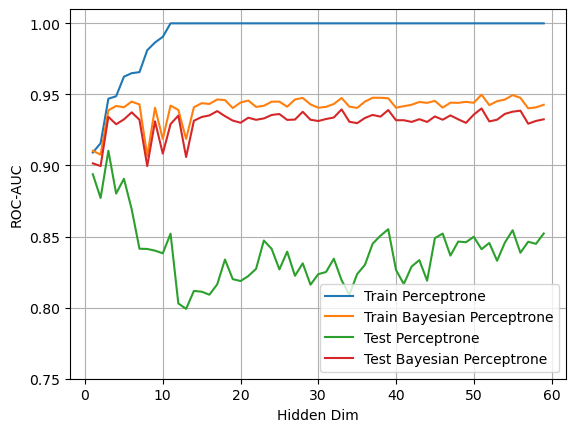
\includegraphics[width=1\linewidth]{roc_auc.png}
    \caption{Зависимость $ROC-AUC$ от размерности скрытого состояния на тренировочных и тестовых данных}
    \label{fig:enter-label}
\end{figure}

\section{Выводы}
По результатам работы можно сделать следующие выводы:
\begin{itemize}
    \item с ростом сложности модели байесовская нейронная сеть не переобучилась;
    \item значение ROC-AUC на тестовой выборке имеет очень высокую корреляцию со значением ROC-AUC на тренировочной выборке (0.97 по Пирсону). Следовательно, для подбора гиперпараметров можно ориентироваться на метрики, полученные по тренировочной выборке. Это даёт нам возможность отказаться от деления на тренировочную и валидационную выборки для подбора гиперпараметров.
\end{itemize}

Так же стоит отметить, что данный подход переносится на другие архитектуры нейронных сетей (рекуррентные, свёрточные, трансформеры).

Имплементация данного подхода была выполнена с использованием PyTorch. Весь исходный код для проведения экспериментов размещён по адресу \url{https://github.com/dimabasow/bayesian-neural-networks}.

\end{document}
